\chapter{Approximations in Multi-Group Transport Theory}
\label{chap:mgxs}

This chapter presents an overview of some of the approximations made by methods which solve the multi-group form of the neutron transport equation. This chapter begins by reviewing the continuous energy steady-state neutron transport equation in Sec.~\ref{sec:chap2-background}. The following sections present simplifications to the angular (Sec.~\ref{sec:chap2-approx-angle}), energy (Sec.~\ref{sec:chap2-approx-energy}) and spatial dependence (Sec.~\ref{sec:chap2-approx-space}) of the equation. The approximations are not specific to a particular approach for solving the transport equation and may be employed by either stochastic or deterministic methods. Sec.~\ref{sec:chap2-mgxs-lib} concludes with a discussion of how these approximations present challenges for accurate \ac{MGXS} generation.


%%%%%%%%%%%%%%%%%%%%%%%%%%%%%%%%%%%%%%%%%%%%%%%%%%%%%%%%%%%%%%%%%%%%%%%%%%%%%%%
\section{Background}
\label{sec:chap2-background}

The field of reactor physics is concerned with computing the distribution of nuclear reaction rates throughout a nuclear reactor core. Nuclear reaction rates are dependent on two fundamental quantities: the density of neutrons and the probability of interaction. The angular neutron flux $\psi(\mathbf{r},\mathbf{\Omega},E)$ models the neutron density\footnote{Unlike the common definition of flux used in other areas of science and engineering, the angular flux $\psi$ is the product of the volume density and speed of neutrons in phase space.} as the path length traveled by neutrons per unit volume and is dependent on a neutron's spatial position $\mathbf{r}$, direction of motion $\mathbf{\Omega}$ and energy $E$\footnote{Vector-valued quantities are expressed in boldface font.}$^{,}$\footnote{This thesis focuses on steady-state calculations and time dependence is neglected for simplicity.}. The macroscopic cross section $\Sigma_{x}(\mathbf{r},E)$ is defined as the probability of interaction $x$ per unit of length traveled by a neutron at some position and energy. A reaction rate $\mathcal{R}_{x}$ can be simply computed as the product of the angular flux and cross section:

\begin{dmath}
\label{eqn:chap2-rxn-rates}
\mathcal{R}_{x}(\mathbf{r},\mathbf{\Omega},E) = \Sigma_{x}(\mathbf{r},E) \psi(\mathbf{r},\mathbf{\Omega},E)
\end{dmath}

\noindent The macroscopic cross section $\Sigma_{x}$ is proportional to a quantity known as the microscopic cross section $\sigma_{x}$. The microscopic cross section is a property of a particular nuclide and is measured experimentally for various reaction types $x$ which include fission $f$, radiative capture $\gamma$ and scattering $s$\footnote{Scattering as defined here includes both inelastic and elastic scattering channels.}. The macroscopic cross section is the sum of the microscopic cross sections of each nuclide $i$ weighted by its number density $N_{i}$:

\begin{dmath}
\label{eqn:chap2-macro-xs-sum}
\Sigma_{x}(\mathbf{r},E) = \sum_{i}N_{i}(\mathbf{r})\sigma_{i,x}(E)
\end{dmath}

The microscopic cross section is highly dependent on the energy of the incoming neutron. As illustrated in Fig.~\ref{fig:chap2-u238-xs}, a cross section varies several orders of magnitude within an energy interval on the order of an eV near nuclear resonances. The probability of some interactions also depends on other properties which characterize the output channel of the reaction. For example, the scattering cross section $\sigma_{s}$ depends on the energy and direction of motion of the outgoing neutron. The macroscopic cross section varies in space when nuclide densities depend on the position within a heterogeneous system.

\begin{figure}[H]
  \centering
  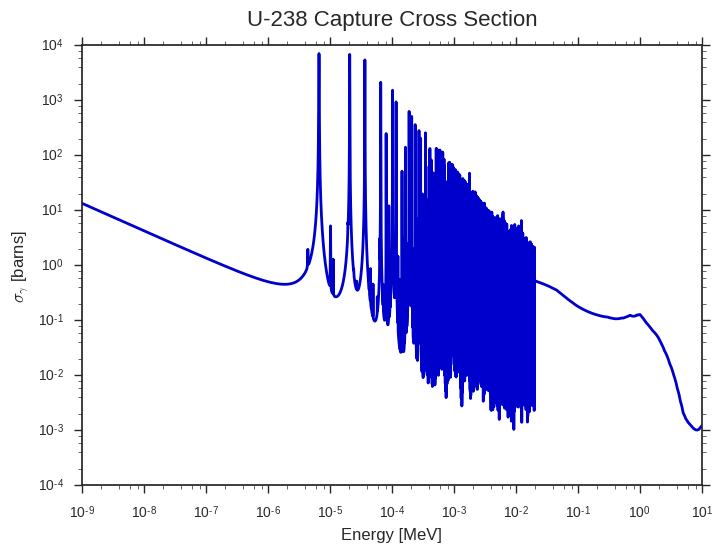
\includegraphics[width=0.8\linewidth]{figures/mgxs/u238-capture-xs}
\caption[U-238 capture cross section]{The continuous energy capture cross section for U-238.}
\label{fig:chap2-u238-xs}
\end{figure}
 
Although cross sections are experimentally measured, the neutron flux must be calculated analytically or with simulation. The steady-state Boltzmann transport equation~\cite{bell1970nuclear} is integro-differential in the neutron angular flux $\psi(\mathbf{r},\mathbf{\Omega},E)$ and balances the rate of change of the population of neutrons in phase space to the difference between the production and loss rates of neutrons within a closed system:

\begin{dmath}
\label{eqn:chap2-transport-ce}
\mathbf{\Omega} \cdot \nabla \psi(\mathbf{r},\mathbf{\Omega},E) + \Sigma_{t}(\mathbf{r},E)\psi(\mathbf{r},\mathbf{\Omega},E) \;\;\;\;\; = \;\;\;\;\; \int\displaylimits_{0}^{\infty}\int\displaylimits_{4\pi} \Sigma_{s}(\mathbf{r},{\mathbf{\Omega'}\rightarrow\mathbf{\Omega}},{E'\rightarrow E}) \psi(\mathbf{r},\mathbf{\Omega'},E') \mathrm{d}\mathbf{\Omega'} \mathrm{d}E' + Q(\mathbf{r},\mathbf{\Omega},E)
\end{dmath}

The first term on the left hand side of the equation represents the streaming of neutrons within space and the second term is the total neutron collision rate determined by the total cross section $\Sigma_{t}$. On the right hand side, the first term models the scattering of neutrons at some energy $E'$ and direction $\mathbf{\Omega'}$ into energy $E$ and direction $\mathbf{\Omega}$. The final term represents a generic source $Q$ of neutrons. In the case of critical systems, such as nuclear reactors, $Q$ is a source of fission neutrons:

\begin{dmath}
\label{eqn:chap2-source}
Q(\mathbf{r},\mathbf{\Omega},E) = \frac{1}{k_{eff}}\int\displaylimits_{0}^{\infty}\int\displaylimits_{4\pi} \nu\Sigma_{f}(\mathbf{r},{\mathbf{\Omega'}\rightarrow \mathbf{\Omega}},{E'\rightarrow E})\psi(\mathbf{r},\mathbf{\Omega'},E') \mathrm{d}\mathbf{\Omega'} \mathrm{d}E'
\end{dmath}

\noindent The fission production cross section $\nu\Sigma_{f}$ represents the probability of neutrons emitted at energy $E$ and angle $\mathbf{\Omega}$ resulting from fission events precipitated by neutrons at $E'$ and $\mathbf{\Omega'}$. The eigenvalue $k_{eff}$ of a critical system represents the multiplication of neutrons from fission and forces balance between neutron sources and losses due to absorption and leakage.

A solution for the neutron flux must computed from the transport equation in order to compute reaction rate distributions. The accurate determination of the neutron flux is primarily challenged by  the complicated energy structure of the cross sections. In addition, the distribution of neutrons in \ac{LWR}s spans 11 orders of magnitude from a few MeV at birth from fission emission to death by absorption at energies as low as 10$^{-5}$ eV. As a result, analytical solutions to Eqn.~\ref{eqn:chap2-transport-ce} are intractable without significant simplifying assumptions.

Instead, numerical simulation is used to solve the transport equation for the flux. Monte Carlo may be employed to exactly treat the energy dependence in Eqn.~\ref{eqn:chap2-transport-ce}\footnote{The treatment is only as exact as the uncertainties in measured nuclear cross section data will permit.}, but it is computationally burdensome and impractical for routine nuclear reactor analysis. Although space and angle may be discretized using standard techniques for the solution of partial differential equations, special treatment must be given to the energy variable. The following sections introduce approximations used to reduce the dimensionality of the equation to permit tractable multi-group calculations.

\begin{emphbox}
\textbf{Nuclear reactor simulations calculate the neutron multiplication factor $k_{eff}$ and reaction rate spatial distributions. Monte Carlo methods are the most accurate approach, but are not yet practical for full-core analysis.}
\end{emphbox}

%The following sections present standard approximations made in multi-group theory to reduce the dimensionality of the angular, energy and spatial variables 


%%%%%%%%%%%%%%%%%%%%%%%%%%%%%%%%%%%%%%%%%%%%%%%%%%%%%%%%%%%%%%%%%%%%%%%%%%%%%%%
\section{Approximations in Angle}
\label{sec:chap2-approx-angle}

%%%%%%%%%%%%%%%%%%%%%%%%%%%
\subsection{Isotropic Fission Source}
\label{subsec:chap2-fiss-src}

The neutrons emitted from fission form a nearly isotropic distribution independent of the energy or angle of the incoming neutron\footnote{This approximation is only valid for a large number of fission events as is the case in a nuclear reactor.}. As a result, the fission production cross section can be approximated as $\nu\Sigma_{f}(\mathbf{r},{\mathbf{\Omega'}\rightarrow \mathbf{\Omega}},{E'\rightarrow E}) \approx \nu\Sigma_{f}(\mathbf{r},{E'\rightarrow E})$. This permits the fission source in Eqn.~\ref{eqn:chap2-source} to be written as:

\begin{dmath}
\label{eqn:chap2-source-scalar-flux}
Q(\mathbf{r},\mathbf{\Omega},E) = \frac{1}{4\pi k_{eff}}\int\displaylimits_{0}^{\infty}\int\displaylimits_{4\pi} \nu\Sigma_{f}(\mathbf{r},{E'\rightarrow E})\psi(\mathbf{r},\mathbf{\Omega},E') \mathrm{d}\mathbf{\Omega} \mathrm{d}E'
\end{dmath}

\noindent This expression may be further simplified in terms of the scalar neutron flux $\phi(\mathbf{r},E)$:

\begin{dmath}
\label{eqn:chap2-source-scalar-flux}
Q(\mathbf{r},\mathbf{\Omega},E) = \frac{1}{4\pi k_{eff}} \int\displaylimits_{0}^{\infty}\nu\Sigma_{f}(\mathbf{r},{E'\rightarrow E})\phi(\mathbf{r},E') \mathrm{d}E'
\end{dmath}

\begin{dmath}
\label{eqn:chap2-scalar-flux}
\phi_{g}(\mathbf{r},E) = \int\displaylimits_{4\pi}\psi(\mathbf{r},\mathbf{\Omega},E)\mathrm{d}\mathbf{\Omega}
\end{dmath}

\noindent The isotropic approximation reduces the dimensionality of the fission production term in the transport equation and simplifies the derivation of the approximations in the following sections.


%%%%%%%%%%%%%%%%%%%%%%%%%%%%%%
\subsection{Angular Expansion of the Scattering Kernel}
\label{subsec:chap2-scatt-src}

Unlike the fission source, the source of neutrons from scattering cannot be treated as isotropic since it is strongly dependent on the relationship between the incoming and outgoing directions of motion. The dimensionality of the scattering source term in the transport equation -- known as the double differential scattering kernel -- is commonly reduced with basis function expansions in angle~\cite{hebert2009applied, cacuci2010handbook}. The angular flux is first expanded as an infinite sum of spherical harmonic functions $Y_{\ell}^{m}(\mathbf{\Omega})$ and angular flux moments $\psi_{\ell}^{m}(\mathbf{r},E)$:

\begin{dmath}
\label{eqn:chap2-flux-expand}
\psi(\mathbf{r},\mathbf{\Omega},E) = \displaystyle\sum\limits_{\ell=0}^{\infty} \frac{2\ell+1}{4\pi} \displaystyle\sum\limits_{m=-\ell}^{\ell} \psi_{\ell}^{m}(\mathbf{r},E)Y_{l}^{m}(\mathbf{\Omega})
\end{dmath}

\begin{dmath}
\label{eqn:chap2-flux-moment}
\psi_{\ell}^{m}(\mathbf{r},E) = \displaystyle\int\limits_{4\pi} \psi(\mathbf{r},\mathbf{\Omega},E)Y_{\ell}^{m}(\mathbf{\Omega}) \mathrm{d}\mathbf{\Omega}
\end{dmath}

Similarly, the angular dependence of the scattering cross section $\Sigma_{s}(\mathbf{r},{\mathbf{\Omega'}\rightarrow\mathbf{\Omega}},{E'\rightarrow E})$ can be treated with a basis function expansion. The scattering cross section can be simplified without approximation by noting that the distribution over the change in direction $\mu$ is independent of the incoming angle $\mathbf{\Omega'}$ in isotropic media. The re-parametrized scattering cross section $\Sigma_{s}(\mathbf{r},\mu,E'\rightarrow E)$ can then be expanded as an infinite sum of Legendre polynomials $P_{\ell}(\mu)$ and scattering moments $\Sigma_{s,\ell}(\mathbf{r},{E'\rightarrow E})$:

\begin{dmath}
\label{eqn:chap2-scatt-expand}
\Sigma_{s}(\mathbf{r},\mu,E'\rightarrow E) = \displaystyle\sum\limits_{\ell=0}^{\infty} \frac{2\ell+1}{2} \Sigma_{s,\ell}(\mathbf{r},{E'\rightarrow E})P_{\ell}(\mu)
\end{dmath}

\begin{dmath}
\label{eqn:chap2-scatt-moment}
\Sigma_{s,\ell}(\mathbf{r},E'\rightarrow E) = \displaystyle\int\limits_{-1}^{1} \Sigma_{s}(\mathbf{r},\mu,{E'\rightarrow E})P_{\ell}(\mu)\mathrm{d}\mu
\end{dmath}

The expansions of the angular flux in spherical harmonics and the scattering cross section in Legendre polynomials may be substituted into the scattering kernel. The spherical harmonic addition theorem can be applied to simplify the kernel in terms of only the real components $R_{\ell}^{m}(\mathbf{\Omega})$ of the spherical harmonics:

\begin{dmath}
\label{eqn:chap2-scatt-src-expand}
\int\displaylimits_{0}^{\infty}\int\displaylimits_{4\pi} \Sigma_{s}(\mathbf{r},{\mathbf{\Omega'}\rightarrow\mathbf{\Omega}},{E'\rightarrow E}) \psi(\mathbf{r},\mathbf{\Omega'},E') \mathrm{d}\mathbf{\Omega'} \mathrm{d}E' = \int\displaylimits_{0}^{\infty} \displaystyle\sum\limits_{\ell=0}^{\infty} \frac{2\ell+1}{4\pi} \Sigma_{s,\ell}(\mathbf{r},{E'\rightarrow E}) \psi_{\ell}^{m}(\mathbf{r},E')R_{\ell}^{m}(\mathbf{\Omega}) \mathrm{d}E'
\end{dmath}

No approximation has been made to the scattering kernel's angular dependence in Eqn.~\ref{eqn:chap2-scatt-src-expand}. In practice, however, the expansion is truncated to a finite number of spherical harmonics $L$ to make the transport equation computationally tractable. The transport equation with the scattering source expansion and isotropic fission source is then:

\begin{dmath}
\label{eqn:chap2-transport-ce-2}
\mathbf{\Omega} \cdot \nabla \psi(\mathbf{r},\mathbf{\Omega},E) + \Sigma_{t}(\mathbf{r},E)\psi(\mathbf{r},\mathbf{\Omega},E) = \int\displaylimits_{0}^{\infty} \displaystyle\sum\limits_{\ell=0}^{L} \frac{2\ell+1}{4\pi} \displaystyle\sum\limits_{m=-\ell}^{\ell} \Sigma_{s,\ell}(\mathbf{r},{E'\rightarrow E}) \psi_{\ell}^{m}(\mathbf{r},E')R_{\ell}^{m}(\mathbf{\Omega}) \mathrm{d}E' + \frac{1}{4\pi k_{eff}}\int\displaylimits_{0}^{\infty} \nu\Sigma_{f}(\mathbf{r},{E'\rightarrow E})\phi(\mathbf{r},E')\mathrm{d}E'
\end{dmath}


%%%%%%%%%%%%%%%%%%%%%%%%%%%%%%
\subsection{Transport Correction}
\label{subsec:chap2-transport-corr}

The scattering matrix and flux moments substantially increase the memory and storage requirements for calculation schemes which model anisotropic scattering with a finite moment expansion as introduced in Sec.~\ref{subsec:chap2-scatt-src}. In practice, many methods attempt to implicitly model anisotropic scattering effects with transport corrected cross sections. These approaches seek to define a correction which makes the transport equation with isotropic scattering in the laboratory system ($L=0$) equivalent to the general equation with anisotropic scattering. Various transport corrections are thoroughly detailed in the TRANSX~\cite{macfarlane1993transx} and NJOY~\cite{macfarlane2000njoy} manuals, each of which follows the approach taken by Bell, Hansen and Sandmeier in~\cite{bell1967transport}. This section summarizes the derivation in~\cite{hebert2009applied}.

First, consider a truncated form of the Legendre polynomial expansion of the scattering cross section $\Sigma_{s}(\mathbf{r},\mu,E'\rightarrow E)$ in Eqn.~\ref{eqn:chap2-scatt-expand}:

\begin{dmath}
\label{eqn:chap2-scatt-expand-truncate}
\Sigma_{s}(\mathbf{r},\mu,E'\rightarrow E) = \displaystyle\sum\limits_{\ell=0}^{\infty} \frac{2\ell+1}{2} \Sigma_{s,\ell}(\mathbf{r},{E'\rightarrow E})P_{\ell}(\mu) \approx \displaystyle\sum\limits_{\ell=0}^{L} \frac{2\ell+1}{2} \tilde{\Sigma}_{s,\ell}(\mathbf{r},{E'\rightarrow E})P_{\ell}(\mu) + \Delta\Sigma_{tr}(\mathbf{r},{E'\rightarrow E})\delta(\mu-1)
\end{dmath}

\noindent where $\tilde{\Sigma}_{s,\ell}$ is a modified form of the scattering moment $\Sigma_{s,\ell}$ and $\Delta\Sigma_{tr}$ is a transport correction term. The Kronecker delta function $\delta(\mu-1)$ is used to make the correction term forward peaked in order to best capture the first order anisotropies in thermal reactors. The coefficients $\tilde{\Sigma}_{s,\ell}$ and $\Delta\Sigma_{tr}$ are defined such that the Legendre moments of the scattering cross section in Eqn.~\ref{eqn:chap2-scatt-moment} are preserved for $0 \le \ell \le L+1$:

\begin{dmath}
\label{eqn:chap2-scatt-moment-preserve}
\Sigma_{s,\ell}(\mathbf{r},E'\rightarrow E) = \displaystyle\int\limits_{-1}^{1} \Sigma_{s}(\mathbf{r},\mu,{E\rightarrow E})P_{\ell}(\mu)\mathrm{d}\mu \approx \displaystyle\int\limits_{-1}^{1} \displaystyle\sum\limits_{\ell'=0}^{L} \frac{2\ell'+1}{2} \tilde{\Sigma}_{s,\ell'}(\mathbf{r},{E'\rightarrow E})P_{\ell'}(\mu)P_{\ell}(\mu)\mathrm{d}\mu + \displaystyle\int\limits_{-1}^{1} \Delta\Sigma_{tr}(\mathbf{r},{E'\rightarrow E})\delta(\mu-1)P_{\ell}(\mu)\mathrm{d}\mu
\end{dmath}

The following simultaneous system of equalities for $0 \le \ell \le L$ follows from the identity $P_{\ell}(1) = 1$ and the orthogonality relation of the Legendre polynomial basis set:

\begin{dmath}
\label{eqn:chap2-sigsl}
\tilde{\Sigma}_{s,\ell}(\mathbf{r},{E'\rightarrow E}) + \Delta\Sigma_{tr}(\mathbf{r},{E'\rightarrow E}) = \Sigma_{s,\ell}(\mathbf{r},{E'\rightarrow E})
\end{dmath}

\begin{dmath}
\label{eqn:chap2-delta-transport}
\Delta\Sigma_{tr}(\mathbf{r},{E'\rightarrow E}) = \Sigma_{s,L+1}(\mathbf{r},{E'\rightarrow E})
\end{dmath}

\noindent For isotropic in lab scattering with $L = 0$ the Eqns.~\ref{eqn:chap2-scatt-expand-truncate} and~\ref{eqn:chap2-delta-transport} simplify in terms of only the zeroth and first order scattering moments:

\begin{dmath}
\label{eqn:chap2-iso-scatt-kernel-transport}
\Sigma_{s}(\mathbf{r},\mu,E'\rightarrow E) \approx \frac{1}{2}\left[\Sigma_{s,0}(\mathbf{r},{E'\rightarrow E}) - \Sigma_{s,1}(\mathbf{r},{E'\rightarrow E})\right] + \Sigma_{s,1}(\mathbf{r},{E'\rightarrow E})\delta(\mu-1)
\end{dmath}

\noindent The transport-corrected scattering cross section in Eqn.~\ref{eqn:chap2-iso-scatt-kernel-transport} is then substituted into the transport equation in Eqn.~\ref{eqn:chap2-transport-ce-2} with an isotropic scattering kernel and rearranged to produce:

\begin{dmath}
\label{eqn:chap2-transport-ce-3}
\mathbf{\Omega} \cdot \nabla \psi(\mathbf{r},\mathbf{\Omega},E) + \Sigma_{t}(\mathbf{r},E)\psi(\mathbf{r},\mathbf{\Omega},E) - \int\displaylimits_{0}^{\infty} \Sigma_{s,1}(\mathbf{r},{E'\rightarrow E})\phi(\mathbf{r},E')\mathrm{d}E' = \frac{1}{4\pi} \int\displaylimits_{0}^{\infty} \left[\Sigma_{s,0}(\mathbf{r},{E'\rightarrow E}) - \Sigma_{s,1}(\mathbf{r},{E'\rightarrow E})\right] \phi(\mathbf{r},E')\mathrm{d}E' + \frac{1}{4\pi k_{eff}}\int\displaylimits_{0}^{\infty}\nu\Sigma_{f}(\mathbf{r},{E'\rightarrow E})\phi(\mathbf{r},E') \mathrm{d}E'
\end{dmath}

\noindent where the relation $\phi = \psi_{0}^{0}$ for the scalar flux has been used to completely remove the angular dependence from the isotropic scattering kernel. The transport correction term $\Delta\Sigma_{tr}(\mathbf{r},E)$ can be defined such that it can be lumped into new transport-corrected total and scattering cross sections $\tilde{\Sigma}_{t}$ and $\tilde{\Sigma}_{s}$ as follows:

\begin{dmath}
\label{eqn:chap2-transport-xs}
\Delta\Sigma_{tr}(\mathbf{r},E) \equiv \frac{\int\displaylimits_{0}^{\infty} \Sigma_{s,1}(\mathbf{r},{E'\rightarrow E})\phi(\mathbf{r},E') \mathrm{d}E'}{\phi(\mathbf{r},E)}
\end{dmath}

\begin{dmath}
\label{eqn:chap2-transpot-corr-tot-x}
\tilde{\Sigma}_{t}(\mathbf{r},E) = \Sigma_{t}(\mathbf{r},E) - \Delta\Sigma_{tr}(\mathbf{r},E)
\end{dmath}

\begin{dmath}
\label{eqn:chap2-transpot-corr-scatt-x}
\tilde{\Sigma}_{s}(\mathbf{r},{E'\rightarrow E}) = \Sigma_{s,0}(\mathbf{r},{E'\rightarrow E}) - \Delta\Sigma_{tr}(\mathbf{r},E)\delta(E'-E)
\end{dmath}

This definition of the transport correction is termed the \textit{in-scatter approximation} in the literature~\cite{yamamoto2008simplified}. Finally, the transport equation in Eqn.~\ref{eqn:chap2-transport-ce-3} can be simplified with the substitution of the corrected total and scattering cross sections:

\begin{dmath}
\label{eqn:chap2-transport-ce-4}
\mathbf{\Omega} \cdot \nabla \psi(\mathbf{r},\mathbf{\Omega},E) + \tilde{\Sigma}_{t}(\mathbf{r},E)\psi(\mathbf{r},\mathbf{\Omega},E) = \frac{1}{4\pi} \int\displaylimits_{0}^{\infty} \tilde{\Sigma}_{s}(\mathbf{r},{E'\rightarrow E}) \phi(\mathbf{r},E') \mathrm{d}E' + \frac{1}{4\pi k_{eff}}\int\displaylimits_{0}^{\infty} \nu\Sigma_{f}(\mathbf{r},{E'\rightarrow E})\phi(\mathbf{r},E') \mathrm{d}E'
\end{dmath}

%This is the form of the transport equation that will be used throughout the remainder of this chapter. 

%The approximations in energy and space that will be introduced in the following sections are directly applicable to the transport equation with explicit treatment of anisotropic scattering with a moment expansion as given in Eqn.~\ref{eqn:chap2-transport-ce-2}.

%The angular flux expansion can be substituted into the total collision terminto the total collision term in the transport equation:

%\begin{dmath}
%\label{eqn:chap2-tot-expand}
%\Sigma_{t}(\mathbf{r},E)\psi(\mathbf{r},\mathbf{\Omega},E) = \displaystyle\sum\limits_{\ell=0}^{\infty} \frac{2\ell+1}{4\pi} \displaystyle\sum\limits_{m=-\ell}^{\ell} \Sigma_{t,\ell}^{m}(\mathbf{r},E) \psi_{\ell}^{m}(\mathbf{r},E)Y_{l}^{m}(\mathbf{\Omega})
%\end{dmath}

%\begin{dmath}
%\label{eqn:chap2-tot-moment}
%\Sigma_{t,\ell}^{m}(\mathbf{r},E) = \frac{\Sigma_{t}(\mathbf{r},E)\psi_{\ell}^{m}(\mathbf{r},E)}{\psi_{\ell}^{m}(\mathbf{r},E)}
%\end{dmath}

%model scattering as isotropic in the laboratory system (equivalent to truncating the scattering kernel with $L = 0$) and define a transport correction which makes the transport equation equivalent to one with anisotropic scattering

%The expanded total collision term in Eqn.~\ref{eqn:chap2-tot-expand} can be moved to the right hand side of Eqn.~\ref{eqn:chap2-transport-ce-2}, and with some simplifications, incorporated into the scattering kernel expansion. A new free parameter for the transport-corrected total cross section $\Sigma_{tr}$ is then added as a reaction rate to each side of the transport equation, where the spatial and energy variables have been dropped for simplicity:

%\begin{dmath}
%\label{eqn:chap2-transport-ce-3}
%\mathbf{\Omega} \cdot \nabla \psi + \Sigma_{tr}\psi = \int\displaylimits_{0}^{\infty} \displaystyle\sum\limits_{\ell=0}^{L} \frac{2\ell+1}{4\pi} \displaystyle\sum\limits_{m=-\ell}^{\ell} \left(\Sigma_{s,\ell} - \left(\Sigma_{t,\ell}^{m} - \Sigma_{tr}\right)\delta_{E',E}\right) \psi_{\ell}^{m}R_{\ell}^{m}(\mathbf{\Omega}) \mathrm{d}E' + \frac{1}{4\pi k_{eff}}\int\displaylimits_{0}^{\infty}\int\displaylimits_{4\pi} \nu\Sigma_{f}\psi \mathrm{d}\mathbf{\Omega'} \mathrm{d}E'
%\end{dmath}

%The scattering kernel expansion has been truncated to order $L$ and the variable $\delta_{E',E}$ is the Kronecker delta function. A variety of forms for the transport cross section $\Sigma_{tr}$ are extensively discussed in the literature. One of the most commonly used versions of $\Sigma_{tr}$ is known as the \textit{in-scatter approximation}~\cite{yamamoto2008simplified}. In the case of isotropic scattering where $L = 0$, the in-scatter approximation is defined as the total cross section with a current-weighted correction term based on $\Sigma_{s,\ell=1}$:

%This form is Each of these forms are presented here for the case of isotropic scattering where $L = 0$, as is a common scenario in many deterministic transport codes.

%\begin{dmath}
%\label{eqn:chap2-transport-in-scatt-curr}
%\Sigma_{tr}(\mathbf{r},E) \equiv \Sigma_{t}(\mathbf{r},E) - \frac{\int\limits_{0}^{\infty}\Sigma_{s,\ell=1}(\mathbf{r},{E'\rightarrow E})\psi_{1}(\mathbf{r},E')\mathrm{d}E'}{\psi_{1}(\mathbf{r},E)}
%\end{dmath}

%Since it is generally impractical to compute the neutron current \textit{a priori}, the first moment of the flux -- known as the scalar flux $\phi$ -- is more commonly used to weight the correction term:

%In-scatter approximation with scalar flux weighting - make the approximation that weighting with the current $\psi_{1}$ is akin to weighting with the scalar flux $\psi_{0}$:

%\begin{dmath}
%\label{eqn:chap2-transport-in-scatt-flux}
%\Sigma_{tr}(\mathbf{r},E) \equiv \Sigma_{t}(\mathbf{r},E) - \frac{\int\limits_{0}^{\infty}\Sigma_{s,\ell=1}(\mathbf{r},{E'\rightarrow E})\psi_{0}(\mathbf{r},E')\mathrm{d}E'}{\psi_{0}(\mathbf{r},E)}
%\end{dmath}

%Out-scatter approximation:

%\begin{dmath}
%\label{eqn:chap2-transport-out-scatt}
%\Sigma_{tr}(\mathbf{r},E) \equiv \Sigma_{t}(\mathbf{r},E) - \int\limits_{0}^{\infty}%\Sigma_{s,\ell=1}(\mathbf{r},{E'\rightarrow E})\mathrm{d}E'
%\end{dmath}

%Although some deterministic transport codes explicitly treat the anisotropy of the scattering source with a finite moment expansion, it is common for many methods to assume isotropic scattering and model the first term in the expansion in terms of the scalar neutron flux $\phi$:

%\begin{dmath}
%\label{eqn:chap2-scatt-src-iso}
%\int\displaylimits_{0}^{\infty}\int\displaylimits_{4\pi} \Sigma_{s}(\mathbf{r},{\mathbf{\Omega'}\rightarrow\mathbf{\Omega}},{E'\rightarrow E}) \psi(\mathbf{r},\mathbf{\Omega'},E') \mathrm{d}\mathbf{\Omega'} \mathrm{d}E' \approx \frac{1}{4\pi} \int\displaylimits_{0}^{\infty} \Sigma_{s}(\mathbf{r},{E'\rightarrow E}) \psi_{0}(\mathbf{r},E') = \frac{1}{4\pi} \int\displaylimits_{0}^{\infty} \Sigma_{s,0}(\mathbf{r},{E'\rightarrow E}) \phi(\mathbf{r},E') \mathrm{d}E'
%\end{dmath}

%\begin{dmath}
%\label{eqn:chap2-source-scalar-flux}
%\phi(\mathbf{r},E) = \int\displaylimits_{4\pi}\psi(\mathbf{r},\mathbf{\Omega'},E) \mathrm{d}\Omega'
%\end{dmath}

\begin{emphbox}
\textbf{The neutron fission source is isotropic in reactors. The scattering source is simplified with a basis function expansion in angle. A transport correction is commonly used to account for anisotropic scattering in simulations that simplify the scattering source as isotropic.}
\end{emphbox}


%%%%%%%%%%%%%%%%%%%%%%%%%%%%%%%%%%%%%%%%%%%%%%%%%%%%%%%%%%%%%%%%%%%%%%%%%%%%%%%
\section{Approximations in Energy}
\label{sec:chap2-approx-energy}

%%%%%%%%%%%%%%%%%%%%%%%%%%%%%%%%%%
\subsection{Energy Discretization}
\label{subsec:chap2-energy}

The multi-group approach used to solve the transport equation subdivides the neutron's energy into discrete bins known as energy groups. The energy groups are indexed starting at 1 for high energies and ending with $G$ for the lowest energies of interest. An energy group $g \in \left\{1, 2, \ldots, G\right\}$ spans a range of energies from $\left[E_{g}, E_{g-1}\right]$ where $E_{0}$ is the highest energy under consideration and $E_{g}$ is the upper bound of group $g$\footnote{This convention derives from the fact that neutrons are emitted at high energies from fission and are absorbed at lesser energies in \ac{LWR}s.}. First, a group-wise angular flux $\psi_{g}$ and scalar flux $\phi_{g}$ is defined for each energy group:

\begin{dmath}
\label{eqn:chap2-groupwise-flux-angular}
\psi_{g}(\mathbf{r},\mathbf{\Omega}) = \int\displaylimits_{E_{g}}^{E_{g-1}} \psi(\mathbf{r},\mathbf{\Omega},E)\mathrm{d}E
\end{dmath}

\begin{dmath}
\label{eqn:chap2-groupwise-flux-scalar}
\phi_{g}(\mathbf{r}) = \int\displaylimits_{E_{g}}^{E_{g-1}} \phi(\mathbf{r},E)\mathrm{d}E
\end{dmath}

\noindent The continuous energy transport equation with isotropic fission and scattering sources and transport-corrected cross sections in Eqn.~\ref{eqn:chap2-transport-ce-4} can be transformed into its multi-group form by integrating over each energy group\footnote{The multi-group approximation with energy discretization may be similarly applied to the transport equation in Eqn.~\ref{eqn:chap2-transport-ce-2} if anisotropic scattering is explicitly treated with scattering moments.}:

\begin{dmath}
\label{eqn:chap2-transport-mg-1}
\mathbf{\Omega} \cdot \nabla \psi_{g}(\mathbf{r},\mathbf{\Omega}) + \int\displaylimits_{E_{g}}^{E_{g-1}} \Bigg[\tilde{\Sigma}_{t}(\mathbf{r},E)\psi(\mathbf{r},\mathbf{\Omega},E)\Bigg]\mathrm{d}E = \;\;\; \int\displaylimits_{E_{g}}^{E_{g-1}} \Bigg[\frac{1}{4\pi} \sum_{g'=1}^{G} \int\displaylimits_{E_{g'}}^{E_{g'-1}} \tilde{\Sigma}_{s}(\mathbf{r},{E'\rightarrow E}) \phi(\mathbf{r},E') \mathrm{d}E'\Bigg]\mathrm{d}E + \int\displaylimits_{E_{g}}^{E_{g-1}}\Bigg[\frac{1}{4\pi k_{eff}}\sum_{g'=1}^{G} \int\displaylimits_{E_{g'}}^{E_{g'-1}}\nu\Sigma_{f}(\mathbf{r},{E'\rightarrow E})\phi(\mathbf{r},E')\mathrm{d}E'\Bigg]\mathrm{d}E
\end{dmath}

\noindent The integrals over incoming neutron energy in the scattering kernel and fission source in Eqn.~\ref{eqn:chap2-transport-mg-1} are treated as summations of discrete integrals over each incoming energy group. Although the streaming term is easily expressed in terms of the multi-group flux $\psi_{g}$, the total collision, scattering and fission terms are defined as integral quantities in energy. These three terms can be simplified by multiplying each by unity in the form of $\nicefrac{\psi_{g}}{\psi_{g}}$ and $\nicefrac{\phi_{g}}{\phi_{g}}$:

\begin{dmath}
\label{eqn:chap2-transport-mg-2}
\mathbf{\Omega} \cdot \nabla \psi_{g}(\mathbf{r},\mathbf{\Omega}) + \left[\frac{\int\displaylimits_{E_{g}}^{E_{g-1}} \tilde{\Sigma}_{t}(\mathbf{r},E)\psi(\mathbf{r},\mathbf{\Omega},E)\mathrm{d}E}{\psi_{g}(\mathbf{r},\mathbf{\Omega})}\right]\psi_{g}(\mathbf{r},\mathbf{\Omega}) 
= \;\;\; 
\frac{1}{4\pi} \sum_{g'=1}^{G} \left[\frac{\int\displaylimits_{E_{g}}^{E_{g-1}} \int\displaylimits_{E_{g'}}^{E_{g'-1}} \tilde{\Sigma}_{s}(\mathbf{r},{E'\rightarrow E}) \phi(\mathbf{r},E')\mathrm{d}E'\mathrm{d}E}{\phi_{g'}(\mathbf{r})}\right]\phi_{g'}(\mathbf{r})
+ 
\dfrac{1}{4\pi k_{eff}} \sum_{g'=1}^{G} \left[\frac{\int\displaylimits_{E_{g}}^{E_{g-1}} \int\displaylimits_{E_{g'}}^{E_{g'-1}} \nu\Sigma_{f}(\mathbf{r},{E'\rightarrow E})\phi(\mathbf{r},E') \mathrm{d}E'\mathrm{d}E}{\phi_{g'}(\mathbf{r})}\right]\phi_{g'}(\mathbf{r})
\end{dmath}

\noindent The bracketed terms in Eqn.~\ref{eqn:chap2-transport-mg-2} are defined as the \ac{MGXS} for total, scattering and fission production reactions. The \ac{MGXS} are the averages of the corresponding continuous energy cross sections weighted by the angular neutron flux $\psi$ in each energy group. The \ac{MGXS} $\tilde{\Sigma}_{t,g}$, $\tilde{\Sigma}_{s,g' \rightarrow g}$ and $\nu\Sigma_{f,g' \rightarrow g}$ are defined below for completeness:

\begin{dmath}
\label{eqn:chap2-sigt-mg}
\tilde{\Sigma}_{t,g}(\mathbf{r},\mathbf{\Omega}) \equiv \frac{\int\displaylimits_{E_{g}}^{E_{g-1}} \tilde{\Sigma}_{t}(\mathbf{r},E)\psi(\mathbf{r},\mathbf{\Omega},E)\mathrm{d}E}{\psi_{g}(\mathbf{r},\mathbf{\Omega})}
\end{dmath}

\begin{dmath}
\label{eqn:chap2-sigs-mg}
\tilde{\Sigma}_{s,g' \rightarrow g}(\mathbf{r}) \equiv \frac{\int\displaylimits_{E_{g}}^{E_{g-1}} \int\displaylimits_{E_{g'}}^{E_{g'-1}} \tilde{\Sigma}_{s}(\mathbf{r},{E'\rightarrow E}) \phi(\mathbf{r},E') \mathrm{d}E' \mathrm{d}E} {\phi_{g'}(\mathbf{r})}
\end{dmath}

\begin{dmath}
\label{eqn:chap2-nusigf-mg}
\nu\Sigma_{f,g' \rightarrow g}(\mathbf{r}) \equiv \frac{\int\displaylimits_{E_{g}}^{E_{g-1}} \int\displaylimits_{E_{g'}}^{E_{g'-1}} \nu\Sigma_{f}(\mathbf{r},{E'\rightarrow E})\phi(\mathbf{r},E') \mathrm{d}E'\mathrm{d}E}{\phi_{g'}(\mathbf{r})}
\end{dmath}

With these definitions of the \ac{MGXS}, the multi-group form of the transport equation in Eqn.~\ref{eqn:chap2-transport-mg-1} can be expressed succinctly in terms of the group-wise fluxes:

\begin{dmath}
\label{eqn:chap2-transport-mg-3}
\mathbf{\Omega} \cdot \nabla \psi_{g}(\mathbf{r},\mathbf{\Omega}) + \tilde{\Sigma}_{t,g}(\mathbf{r},\mathbf{\Omega})\psi_{g}(\mathbf{r},\mathbf{\Omega}) =
\frac{1}{4\pi}\sum_{g'=1}^{G} \tilde{\Sigma}_{s,g' \rightarrow g}(\mathbf{r}) \phi_{g'}(\mathbf{r}) + \frac{1}{4\pi k_{eff}}\sum_{g'=1}^{G} \nu\Sigma_{f,g' \rightarrow g}(\mathbf{r})\phi_{g'}(\mathbf{r})
\end{dmath}

Thus far, no approximations have been made in the energy discretization of multi-group transport equation given in Eqn.~\ref{eqn:chap2-transport-mg-3}. However, the expression for the total multi-group cross section $\tilde{\Sigma}_{t,g}$ in Eqn.~\ref{eqn:chap2-sigt-mg} presents a complication since it is dependent on the unknown angular flux. One common approximation used to eliminate the angular dependence is presented in the following section.

%The transport correction term introduced in Eqn.~\ref{eqn:chap2-transport-xs} may be similarly discretized for each energy group. However, the correction term $\Delta\Sigma_{tr}$ should be weighted with the first order Legendre moment of the flux, or the volumetric neutron current, rather than the scalar flux in order to preserve reaction rates:

%\begin{dmath}
%\label{eqn:chap2-sigtr-mg-1}
%\Delta\Sigma_{tr,g}(\mathbf{r}) \equiv \frac{\int\displaylimits_{E_{g}}^{E_{g-1}} \tilde{\Sigma}_{t}(\mathbf{r},E)\psi_{\ell=1}(\mathbf{r},\mathbf{\Omega},E)\mathrm{d}E}{\psi_{\ell=1,g}(\mathbf{r},\mathbf{\Omega})}
%\end{dmath}

%In practice, the scalar neutron flux is often used instead to condense $\Delta\Sigma_{tr,g}(\mathbf{r})$ in energy since it is often more challenging to estimate the current than the flux:

%NOTE: It is unclear whether the first order Legendre moment of the flux should be used to weight the MG transport correction. This makes sense in 1D, but in 3D we expand the flux in spherical harmonics, so the flux moments have (l,m) indices, and there is no single "neutron current" per se.


%%%%%%%%%%%%%%%%%%%%%%%%%%%%%%
\subsection{Flux Separability Approximation}
\label{subsec:chap2-angle}

The angular dependence of the total cross section is often treated with the flux separability approximation. Flux separability makes the simplifying assumption that the energy and angular dependence of the flux varies independently such that the angular flux can be written as the product of the scalar neutron flux $\phi(\mathbf{r},E)$ and some function $W(\mathbf{r}, \mathbf{\Omega})$:

\begin{dmath}
\label{eqn:chap2-flux-separate}
\psi(\mathbf{r},\mathbf{\Omega},E) = \phi(\mathbf{r},E) W(\mathbf{r},\mathbf{\Omega})
\end{dmath}

\noindent The angular dependence of the $\tilde{\Sigma}_{t,g}$ may then be eliminated by inserting Eqn.~\ref{eqn:chap2-flux-separate} into Eqn.~\ref{eqn:chap2-sigt-mg}, factoring out $W(\mathbf{r},\mathbf{\Omega})$ and writing $\tilde{\Sigma}_{t}$ in terms of the scalar flux:

\begin{dmath}
\label{eqn:chap2-sigt-mg-scalar}
\tilde{\Sigma}_{t,g}(\mathbf{r}) \equiv \frac{\int\displaylimits_{E_{g}}^{E_{g-1}} \tilde{\Sigma}_{t}(\mathbf{r},E)\phi(\mathbf{r},E)W(\mathbf{r},\mathbf{\Omega})\mathrm{d}E}{\phi_{g}(\mathbf{r})W(\mathbf{r},\mathbf{\Omega})} = \frac{\int\displaylimits_{E_{g}}^{E_{g-1}} \tilde{\Sigma}_{t}(\mathbf{r},E)\phi(\mathbf{r},E)\mathrm{d}E}{\phi_{g}(\mathbf{r})}
\end{dmath}

Although flux separability is a simple and commonly used approach to reduce the complexity of the ``true'' multi-group total cross section, it is not always valid and may not preserve neutron balance. The impact of the flux separability approximation is systematically investigated and quantified in Secs.~\ref{chap:biases} and~\ref{chap:sph} for some simple \ac{PWR} benchmark models.

%\begin{dmath}
%\label{eqn:chap2-sigt-mg-scalar}
%\tilde{\Sigma}_{t,g}(\mathbf{r}) \equiv \frac{\int\displaylimits_{E_{g}}^{E_{g-1}} \tilde{\Sigma}_{t}(\mathbf{r},E)\phi(\mathbf{r},E)\mathrm{d}E}{\phi_{g}(\mathbf{r})}
%\end{dmath}

%\begin{dmath}
%\label{eqn:chap2-sigs-mg-scalar}
%\tilde{\Sigma}_{s,0,g' \rightarrow g}(\mathbf{r}) \equiv \frac{\int\displaylimits_{E_{g}}^{E_{g-1}} \int\displaylimits_{E_{g'}}^{E_{g'-1}} \tilde{\Sigma}_{s,0}(\mathbf{r},{E'\rightarrow E}) \phi(\mathbf{r},E') \mathrm{d}E' \mathrm{d}E} {\phi_{g'}(\mathbf{r})}
%\end{dmath}

%\begin{dmath}
%\label{eqn:chap2-nusigf-mg-scalar}
%\nu\Sigma_{f,g' \rightarrow g}(\mathbf{r}) \equiv \frac{\int\displaylimits_{E_{g}}^{E_{g-1}} \int\displaylimits_{E_{g'}}^{E_{g'-1}} \nu\Sigma_{f}(\mathbf{r},{E'\rightarrow E})\phi(\mathbf{r},E') \mathrm{d}E'\mathrm{d}E}{\phi_{g'}(\mathbf{r})}
%\end{dmath}

%The group-wise scalar flux $\phi_{g}$ is the corollary to its angle dependent counterpart $\psi_{g}$:

%\begin{dmath}
%\label{eqn:chap2-scalar-flux-mg}
%\phi_{g}(\mathbf{r}) = \int\displaylimits_{E_{g}}^{E_{g-1}}\phi(\mathbf{r},E)\mathrm{d}E
%\end{dmath}


%%%%%%%%%%%%%%%%%%%%%%%%%%%%%%%%%%%
\subsection{Scattering Production}
\label{sec:chap2-scatt-prod}

Although neutron production is dominated by fission in nuclear reactors, there may also be non-negligible production of neutrons due to scattering multiplicity $(n,xn)$ reactions. Production from scattering is typically accounted for with a factor $\nu_{scatt,g' \rightarrow g}$ which represents the average number of neutrons produced in a scattering reaction. The factor $\nu_{scatt,g' \rightarrow g}$ may be lumped into the scattering matrix $\nu_{scatt,g' \rightarrow g}\Sigma_{s,g' \rightarrow g}$ and substituted directly into the scattering source term in the multi-group transport equation\footnote{It should be noted that $(n,xn)$ reactions typically have different angular and energy distributions than those used to treat $(n,n)$ scattering reactions. Although the energy dependence may be lumped into the multi-group scattering matrix, the angular dependence must be embedded in the angular expansion of the scattering kernel.}.

The $k_{eff}$ eigenvalue is only defined for the fission operator in the transport equation. As a result, deterministic methods which compute the eigenvalue using the fission production, absorption and leakage rates will fail to capture scattering production in the multiplication factor. In order to account for $(n,xn)$ reactions, a ``corrected'' absorption cross section $\tilde{\Sigma}_{a,g} = \Sigma_{a,g} - (\nu_{scatt,g' \rightarrow g} - 1)\Sigma_{s,g' \rightarrow g}$ must be used to preserve neutron balance. Alternatively, $(n,xn)$ reactions will be accounted for if the eigenvalue is computed as the ratio of successive fission sources in iterative deterministic methods.


%%%%%%%%%%%%%%%%%%%%%%%%%%%%%%%%%%%
\subsection{Fission Matrix Condensation}
\label{sec:chap2-fiss-mat}

The scattering and fission production matrices dominate the memory storage requirements for \ac{MGXS} since they depend on both incoming and outgoing energy groups. In thermal reactors, the energy distribution of neutrons produced in fission is nearly independent of the incoming neutron energy, and the fission production matrix can be condensed into two single dimensional vectors for each energy group. The fission spectrum $\chi_{g}$ is introduced as a probability distribution over outgoing fission energies:

\begin{dmath}
\label{eqn:chap2-chi}
\chi_{g} \equiv \frac{\displaystyle\sum\limits_{g'=1}^{G}\nu\Sigma_{f,g'\rightarrow g}\phi_{g'}}{\displaystyle\sum\limits_{g=1}^{G}\displaystyle\sum\limits_{g'=1}^{G}\nu\Sigma_{f,g'\rightarrow g}\phi_{g'}}
\end{dmath}

The group-wise fission production cross section $\nu\Sigma_{f,g'}$ is defined as the sum of $\nu\Sigma_{f,g'\rightarrow g}$ over all outgoing groups and signifies the probability of fission occurring in group $g$:

\begin{dmath}
\label{eqn:chap2-nusifg}
\nu\Sigma_{f,g'} \equiv \displaystyle\sum\limits_{g'=1}^{G}\nu\Sigma_{f,g'\rightarrow g}
\end{dmath}

\noindent Upon substituting $\chi_{g}$ and $\nu\Sigma_{f,g}$ into Eqn.~\ref{eqn:chap2-transport-mg-3} one obtains:

\begin{dmath}
\label{eqn:chap2-transport-mg-4}
\mathbf{\Omega} \cdot \nabla \psi_{g}(\mathbf{r},\mathbf{\Omega}) + \tilde{\Sigma}_{t,g}(\mathbf{r})\psi_{g}(\mathbf{r},\mathbf{\Omega}) = \frac{1}{4\pi} \sum_{g'=1}^{G} \tilde{\Sigma}_{s,g' \rightarrow g}(\mathbf{r}) \phi_{g}(\mathbf{r}) + \frac{\chi_{g}}{4\pi k_{eff}}\sum_{g'=1}^{G} \nu\Sigma_{f,g'}(\mathbf{r})\phi_{g'}(\mathbf{r})
\end{dmath}

%frequently made in multi-group transport calculations thermal reactor spectra the energy distribution of neutrons produced in fission is nearly independent of the incoming neutron energy.

%to reduce the dimensionality of the fission production matrix $\nu\Sigma_{f,g'\rightarrow g}$. In thermal reactor spectra the energy distribution of neutrons produced in fission is nearly independent of the incoming neutron energy.

\begin{emphbox}
\textbf{The multi-group transport equation is defined in terms of the group-wise fluxes and cross sections. \ac{MGXS} are the flux-weighted averages of the continuous energy cross sections that preserve reaction rates in each group. Flux separability uses the scalar instead of the angular flux to weight the total cross section. The fission matrix is condensed into the fission production cross section and the energy spectrum vectors.}
\end{emphbox}


%%%%%%%%%%%%%%%%%%%%%%%%%%%%%%%%%%%%%%%%%%%%%%%%%%%%%%%%%%%%%%%%%%%%%%%%%%%%%%%
\section{Approximations in Space}
\label{sec:chap2-approx-space}

%%%%%%%%%%%%%%%%%%%%%%%%%%%%%%%%%%%
\subsection{Spatial Homogenization}
\label{subsec:chap2-space}

%Up to this point the \ac{MGXS} have been defined as continuously varying in space. Most deterministic methods solve the multi-group transport equation by discretizing the spatial domain. The following equation introduces an integral over each mesh cell $i$ to each term in the multi-group transport equation:

%\begin{dmath}
%\label{eqn:chap2-transport-mg-4}
%\int\displaylimits_{\mathbf{r} \in V_{i}}\left(\mathbf{\Omega} \cdot \nabla \psi_{g}(\mathbf{r},\mathbf{\Omega}) + \Sigma_{t,g}(\mathbf{r})\psi_{g}(\mathbf{r},\mathbf{\Omega})\right)\mathrm{d}\mathbf{r} \;\;\;\; = \;\;\;\;\; \int\displaylimits_{\mathbf{r} \in V_{i}}\sum_{g'=1}^{G} \int\displaylimits_{4\pi} \Sigma_{s,g' \rightarrow g}(\mathbf{r},{\mathbf{\Omega'}\rightarrow\mathbf{\Omega}}) \psi_{g}(\mathbf{r},\mathbf{\Omega'}) \mathrm{d}\mathbf{\Omega'} \mathrm{d}\mathbf{r} + \frac{1}{4\pi k_{eff}}\int\displaylimits_{\mathbf{r} \in V_{i}}\sum_{g'=1}^{G} \int\displaylimits_{4\pi} \nu\Sigma_{f,g' \rightarrow g}(\mathbf{r})\psi_{g}(\mathbf{r},\mathbf{\Omega'}) \mathrm{d}\mathbf{\Omega'} \mathrm{d}\mathbf{r}
%\end{dmath}

Up to this point, the \ac{MGXS} have been defined as continuously varying in space. In practice, most deterministic methods used to solve the multi-group transport equation make the simplifying assumption that material properties are constant across each spatial mesh cell. Spatial homogenization is used to compute flux-weighted volume-averaged cross sections within each mesh cell $k$ with volume $V_{k}$ as follows:

\begin{dmath}
\label{eqn:chap2-sigt-mg-scalar}
\tilde{\Sigma}_{t,k,g} \equiv \frac{\int\displaylimits_{\mathbf{r} \in V_{k}}\left[\int\displaylimits_{E_{g}}^{E_{g-1}} \tilde{\Sigma}_{t}(\mathbf{r},E)\phi(\mathbf{r},E)\mathrm{d}E\right]\mathrm{d}\mathbf{r}}{\int\displaylimits_{\mathbf{r} \in V_{k}}\phi_{g}(\mathbf{r})\mathrm{d}\mathbf{r}}
\end{dmath}

\begin{dmath}
\label{eqn:chap2-sigs-mg-scalar}
\tilde{\Sigma}_{s,k,g' \rightarrow g} \equiv \frac{\int\displaylimits_{\mathbf{r} \in V_{k}}\left[\int\displaylimits_{E_{g}}^{E_{g-1}} \int\displaylimits_{E_{g'}}^{E_{g'-1}} \tilde{\Sigma}_{s}(\mathbf{r},{E'\rightarrow E}) \phi(\mathbf{r},E') \mathrm{d}E' \mathrm{d}E\right]\mathrm{d}\mathbf{r}}{\int\displaylimits_{\mathbf{r} \in V_{k}}\phi_{g'}(\mathbf{r})\mathrm{d}\mathbf{r}}
\end{dmath}

\begin{dmath}
\label{eqn:chap2-nusigf-mg-scalar}
\nu\Sigma_{f,k,{g'\rightarrow g}} \equiv \frac{\int\displaylimits_{\mathbf{r} \in V_{k}}\left[\int\displaylimits_{E_{g}}^{E_{g-1}} \int\displaylimits_{E_{g'}}^{E_{g'-1}} \nu\Sigma_{f}(\mathbf{r},{E'\rightarrow E})\phi(\mathbf{r},E') \mathrm{d}E'\mathrm{d}E\right]\mathrm{d}\mathbf{r}}{\int\displaylimits_{\mathbf{r} \in V_{k}}\phi_{g'}(\mathbf{r})\mathrm{d}\mathbf{r}}
\end{dmath}

\noindent Spatial homogenization may be applied to compute the fission spectrum $\chi_{k,g}$ from the fission production cross section in Eqn.~\ref{eqn:chap2-nusigf-mg-scalar}. The spatially-homogenized \ac{MGXS} must be appropriately defined to preserve reaction rates such that the following equation holds true for each spatial zone $k$ and energy group $g$:

\begin{dmath}
\label{eqn:chap2-transport-mg-5}
\mathbf{\Omega} \cdot \nabla \psi_{g}(\mathbf{r},\mathbf{\Omega}) + \tilde{\Sigma}_{t,g}\psi_{g}(\mathbf{r},\mathbf{\Omega}) = \frac{1}{4\pi} \sum_{g'=1}^{G} \tilde{\Sigma}_{s,k,g' \rightarrow g}\phi_{g'}(\mathbf{r}) + \frac{\chi_{k,g}}{4\pi k_{eff}}\sum_{g'=1}^{G} \nu\Sigma_{f,k,g'}\phi_{g'}(\mathbf{r})
\end{dmath}

%A variety of discretization schemes may be used to solve the following multi-group transport equation in Eqn.~\ref{eqn:chap2-transport-mg-3}, including the \ac{MOC} and discrete ordinates (S$_N$). For first order discretization schemes in space, the transport equation can be re-written in terms of the volume-averaged group-wise fluxes $\psi_{i,g}$ and the spatially-homogenized \ac{MGXS} in each mesh cell and energy group:

%\begin{dmath}
%\label{eqn:chap2-transport-mg-4}
%\mathbf{\Omega} \cdot \nabla \psi_{i,g}(\mathbf{\Omega}) + \Sigma_{t,i,g}\psi_{i,g}(\mathbf{\Omega}) \;\;\;\; = \;\;\;\;\;
%\sum_{g'=1}^{G} \int\displaylimits_{4\pi} \Sigma_{s,i,g' \rightarrow g}\psi_{i,g}(\mathbf{\Omega'}) \mathrm{d}\mathbf{\Omega'} + 
%\frac{1}{4\pi k_{eff}}\sum_{g'=1}^{G} \int\displaylimits_{4\pi} \nu\Sigma_{f,i,g'}\psi_{i,g}(\mathbf{\Omega'}) \mathrm{d}\mathbf{\Omega'}
%\end{dmath}

\noindent This is the form of the multi-group transport equation solved by the deterministic OpenMOC code in this thesis. 

\begin{emphbox}
\textbf{Spatially-homogenized \ac{MGXS} preserve reaction rates in discrete spatial zones.}
\end{emphbox}


%%%%%%%%%%%%%%%%%%%%%%%%%%%%%%%%%%%%%%%%%%%%%%%%%%%%%%%%%%%%%%%%%%%%%%%%%%%%%%%
\section{MGXS Generation}
\label{sec:chap2-mgxs-lib}

The preceding sections described approximations reducing the dimensionality of the transport equation to permit efficient computational simulation. The solution of the transport equation in Eqn.~\ref{eqn:chap2-transport-mg-5} requires knowledge of the energy condensed and spatially-homogenized \ac{MGXS} in Eqns.~\Crefrange{eqn:chap2-sigt-mg-scalar}{eqn:chap2-nusigf-mg-scalar}. This section describes the challenges to computing \ac{MGXS} and outlines the standard multi-level approach for \ac{MGXS} generation. The chapter concludes with a brief introduction to the potential for Monte Carlo methods as an alternative pathway for accurate \ac{MGXS} generation.


%%%%%%%%%%%%%%%%%%%%%%%
\subsection{Challenges}
\label{subsec:chap2-mgxs-lib-challenges}

%The preceding sections introduced a series of approximations which resulted in multi-group forms of the total, scattering and fission cross sections in Eqns.~\Crefrange{eqn:chap2-sigt-mg-scalar}{eqn:chap2-nusigf-mg-scalar}. 

Given a solution to the transport equation for the multi-group flux, general reaction rate distributions may be computed (\textit{e.g.}, radiative capture, recoverable fission energy) with multi-group cross sections for each nuclide and reaction type of interest. Energy condensation and spatial homogenization may be applied to compute multi-group microscopic cross sections $\sigma_{x,i}$ for each reaction type $x$ and nuclide $i$:

\begin{dmath}
\label{eqn:chap2-micro-sigx}
\sigma_{x,i,k,g} = \frac{\int\displaylimits_{\mathbf{r} \in V_{k}} \int\displaylimits_{E_{g}}^{E_{g-1}} \sigma_{x,i}(\mathbf{r},E)\phi(\mathbf{r},E)\mathrm{d}E\mathrm{d}\mathbf{r}}{\int\displaylimits_{\mathbf{r} \in V_{k}} \int\displaylimits_{E_{g}}^{E_{g-1}} \phi(\mathbf{r},E)\mathrm{d}E\mathrm{d}\mathbf{r}}
\end{dmath}

The accurate determination of \ac{MGXS} depends on an accurate understanding of the spatial and energy dependence of the microscopic cross sections and the flux, each of which is depicted in Fig.~\ref{fig:chap2-mgxs-overlay}. The spatial variation of $\sigma_{x,i}$ is known from the reactor's geometric configuration\footnote{The microscopic cross section $\sigma_{x,i}$ is a property unique to each nuclide and reaction and does not vary in space. However, the volume $V_{k}$ may span different regions which may or may not contain nuclide $n$. The discrete spatial variation in the number density $N_{i}$ may be modeled as $\sigma_{x,i}(\mathbf{r},E) = \sigma_{x,i}(E)\mathbb{1}_{V_{k}}(\mathbf{r})$ with the indicator function $\mathbb{1}_{V_{k}}(mathbf{r})$ equal to 1 if $\mathbf{r} \in V_{k}$ and 0 otherwise.}, and the energy dependence is known from experimental data. However, the spatial and energy dependence of the flux are unknown which presents a ``chicken-or-the-egg'' type of quandary for multi-group calculations. This predicament is aptly described in the NJOY manual~\cite{macfarlane2000njoy}:

\begin{displayquote}
\textit{``Wait a minute,'' you ask, ``the purpose of solving the transport equation is to get the flux, but I have to know the flux to compute the multi-group constants!'' This conundrum is the source of much of the ``art'' in using multi-group methods.}
\end{displayquote}

\begin{figure}[h!]
  \centering
  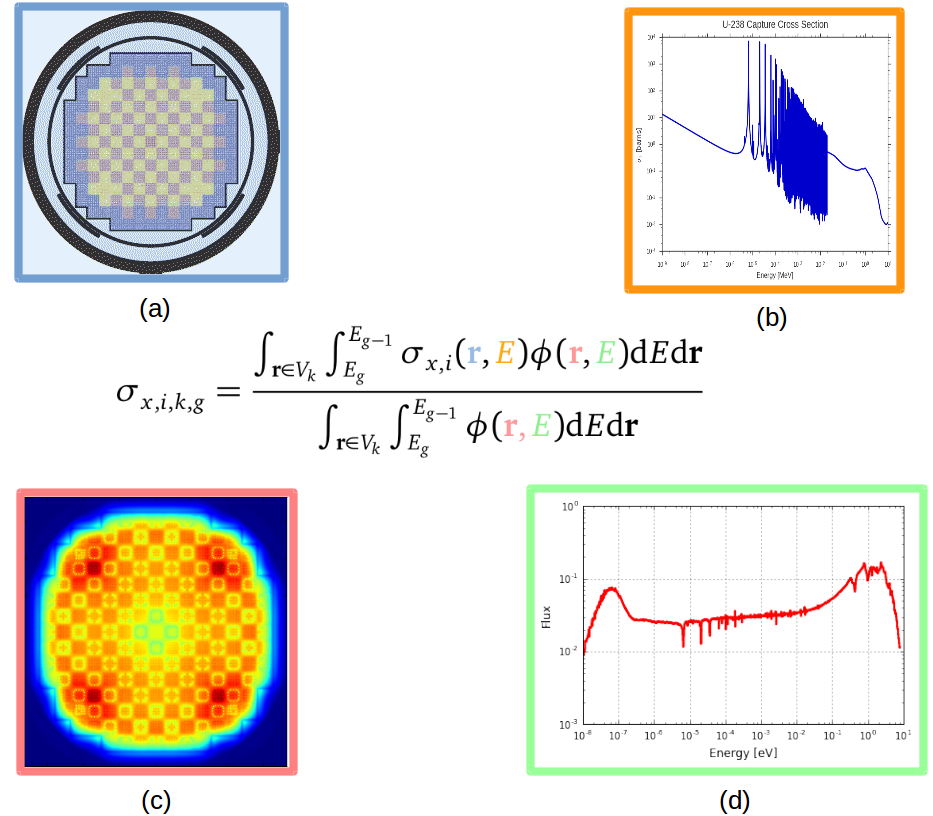
\includegraphics[width=0.9\linewidth]{figures/mgxs/mgxs-overlay}
\caption[Energy and spatial variation in \ac{MGXS}]{The calculation of multi-group cross sections requires knowledge of the spatial and energy variation of the continuous energy cross section and flux. The color-coded position $\mathbf{r}$ and energy $E$ variables correspond to the figures with the matching colored outlines. The microscopic cross section $\sigma_{x,i}$ depends on reactor configuration (a) and neutron energy (b). The flux $\phi$ varies with position (c) and energy (d).}
\label{fig:chap2-mgxs-overlay}
\end{figure}

The \ac{MGXS} are needed to compute the flux, but the flux is needed to compute \ac{MGXS}. As a result, an informed guess is generally made about the flux distribution in order to compute \ac{MGXS}. Such estimates of the flux introduce further approximations in addition to those presented in Secs.~\Crefrange{sec:chap2-approx-angle}{sec:chap2-approx-space}. The following section discusses a high-level overview of the standard multi-level approach to estimating the flux for \ac{MGXS} generation.

%An iterative approach could be used to resolve this issue, but the computational expense would prohibit such a scheme for practical full-core calculations.

%\begin{dmath}
%\label{eqn:chap2-sigt-mg-color}
%\sigma_{x,i,k,g} = \frac{\int\displaylimits_{\mathbf{r} \in V_{k}} \int\displaylimits_{E_{g}}^{E_{g-1}} \sigma_{x,i}(\textcolor{carolinablue}{\mathbf{r}},\textcolor{darktangerine}{E})\phi(\textcolor{lightsalmonpink}{\mathbf{r}},\textcolor{lightgreen}{E})\mathrm{d}E\mathrm{d}\mathbf{r}}{\int\displaylimits_{\mathbf{r} \in V_{k}} \int\displaylimits_{E_{g}}^{E_{g-1}} \phi(\textcolor{lightsalmonpink}{\mathbf{r},\textcolor{lightgreen}{E}})\mathrm{d}E\mathrm{d}\mathbf{r}}
%\end{dmath}

%%%%%%%%%%%%%%%%%%%%%%%%%%%%%%
\subsection{Standard Multi-Level Approach}
\label{subsec:chap2-mgxs-lib-std-approach}

The standard techniques for multi-group cross section generation use a multi-level framework to draw a compromise between accuracy and computational efficiency. The goal in this process is to define a library of \ac{MGXS} which enforces an equivalence between an accurate fine-mesh transport calculation and a corresponding computationally efficient coarse mesh transport or diffusion calculation. The angular, energy and spatial variation of the flux is treated with varying degrees of complexity at each level as illustrated in Fig.~\ref{fig:chap2-mgxs-process}. The process begins with a resonance self-shielding calculation that solves the slowing down problem with point-wise nuclear cross section data in a simple infinite medium, slab or pin cell geometry. The self-shielding calculation produces an \ac{MGXS} library with $\mathcal{O}(100)$ energy groups that is next used by a lattice physics calculation to capture spectral interactions within and between fuel pins in each unique fuel assembly. The lattice physics calculation performs spatial homogenization across each assembly and produces a condensed library with $\mathcal{O}(2-10)$ groups. This assembly-homogenized few group \ac{MGXS} library is finally used by a full-core nodal diffusion calculation.

\begin{figure}[h!]
  \centering
  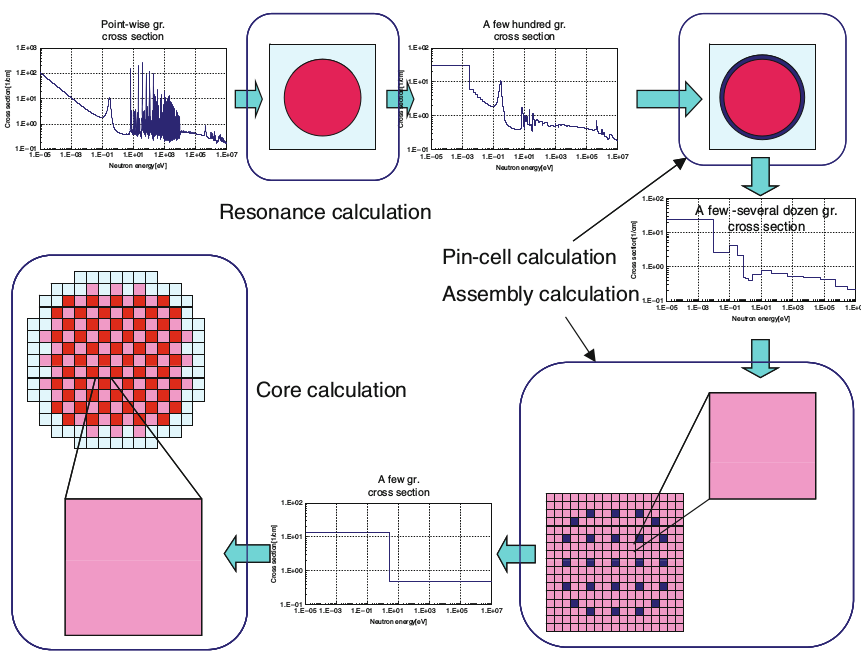
\includegraphics[width=0.9\linewidth]{figures/mgxs/nuke-handbook-mgxs-process}
\caption[Standard multi-level framework for MGXS generation]{The standard multi-level framework for \ac{MGXS} generation taken from the \textit{Handbook of Nuclear Engineering}~\cite{cacuci2010handbook}. The energy dependence of the nuclear cross sections is successively coarsened with resonance self-shielding and lattice physics calculations to generate multi-group libraries for full-core simulations.}
\label{fig:chap2-mgxs-process}
\end{figure}

%The primary challenge throughout this multi-level scheme is to incorporate effects from the resonances in the point-wise cross sections. The spectral interactions which must be accurately accounted for are often referred to as \textit{self-shielding effects} in energy and space. 

The primary challenge throughout this multi-level scheme is to incorporate spectral interactions known as \textit{self-shielding effects} in energy and space. \textit{Energy self-shielding} refers to the impact that resonance interactions may have on the shape of the flux in energy. For example, the sharp depressions in \ac{PWR} flux spectra at energies near the large U-238 thermal capture resonances is an example of energy self-shielding (see Fig.~\ref{fig:chap2-mgxs-overlay}d). These depressions must be accurately captured in the flux used to generate \ac{MGXS}. \textit{Spatial self-shielding} refers to the impact of the material properties in different spatial zones on the flux in other nearby zones. For example, the outer rim of an \ac{LWR} fuel pin shields the center of the pin from neutrons in certain energy groups due to reactions such as U-238 resonance absorption.

%An empty control rod guide tube filled with water, for example, will provide additional moderation and therefore soften the spectrum for nearby fuel pins in \ac{LWR}s, which must be incorporated into the \ac{MGXS} calculation.

There is a long history of approximations for the flux for \ac{MGXS} generation~\cite{cacuci2010handbook}. These include the narrow, wide and intermediate resonance (NR, WR, and IR) approximations used to model the flux in a resonance self-shielding calculation. Lattice physics calculations typically use equivalence in dilution or subgroup methods to model physics in heterogeneous geometries. These approximations are based on simplifying assumptions regarding the geometric configuration, resonance interference effects (mutually overlapping resonances) and temperature distributions\footnote{Although the temperature dependence of cross sections has been neglected thus far for brevity, it must be captured in \ac{MGXS} libraries in order to model Doppler broadening for reactivity coefficient calculations.}. Although ultra-fine methods may be used to compute reference solutions for comparison, they are typically too computationally expensive for routine use. 

As a result of the various approximations employed to model the flux spectrum, the conventional approach for \ac{MGXS} generation is subject to significant engineering prescriptions for different reactor designs.  For example, modifications must be made to lattice physics calculations which account for the impact of local spatial heterogeneities, such as fuel rods adjacent to burnable absorbers. Similarly, it is typical to use infinite boundary conditions (reflective, periodic, white) in resonance self-shielding and lattice physics calculations. This may lead to approximation error in full-core calculations which must model the neutron leakage spectra with vacuum boundary conditions, as well as the flux at the interface between different adjacent assemblies and/or a reflector. As a result, adjustments must be made to the standard multi-level approach in order for the final full-core calculation to accurately account for the effects of spatial heterogeneity.


%%%%%%%%%%%%%%%%%%%%%%%%
\subsection{An Alternative Pathway with Monte Carlo}
\label{subsec:chap2-mgxs-lib-mc}

The multi-level approach of approximations used to generate \ac{MGXS} is the ``Achilles heel'' of multi-group methods. The approximate flux used to compute \ac{MGXS}, along with other approximations inherent in multi-group calculations, require careful use of multi-group methods for reactor analysis. As a result, Monte Carlo must be used to generate reference solutions for benchmarking and verification analysis of multi-group methods. In recent years, there has been growing interest in the use of \ac{MC} in the \ac{MGXS} generation process\cite{leppanen2007serpent,fridman2011serpent,
leppanen2016overview,dorval2015diff,ilas2003monte,pounders2006stochastically,
pounders2009diffusion,pounders2015history,cho2009generation,yun2010monte,
yamamoto2012buckling,yamamoto2012diff,shim2008generation,park2010assembly,park2012generation,
herman2013improved,liuphysor2016,okumura2000validation,tohjoh2005application,
gast1981procedure,ondis2000rcp01,blomquist2002status,redmond1997multigroup,
van2006homogenized,hoogenboom2007generation,yoshioka2010multigroup, yoshioka2011multi,
cai2014condensation,nelson2014improved}. since it offers a potential pathway to use a stochastic approximation to the exact flux in \ac{MGXS} generation.

Continuous energy Monte Carlo is considered the ``gold standard'' for neutron transport calculations since it is reactor agnostic and samples over the entire phase space of angle, energy and position. \ac{MC} is not widely used in routine reactor analysis, however, since its computational expense renders it many orders of magnitude slower than deterministic multi-group methods. Some recent work in the community adopts a hybrid approach which combines the resonance self-shielding and lattice physics stages in a single \ac{MC} simulation. These schemes minimize the computational expense by modeling sub-components (\textit{e.g.}, fuel pins and assemblies) rather than a full reactor. Although the hybrid approach has the advantage of using the ``true'' flux sampled in \ac{MC} to generate \ac{MGXS}, special treatment must still be given to accommodate infinite boundary conditions and neutron leakage spectra.

The following chapter introduces stochastic integration with \ac{MC} and its specific application to compute \ac{MGXS}. In addition, the chapter reviews past and present efforts to generate \ac{MGXS} with \ac{MC} for neutron diffusion and transport codes.


\vfill
\begin{highlightsbox}[frametitle=Highlights]
\begin{itemize}
%  \item Nuclear reactor analysis simulation methods present tradeoffs between accuracy and speed.
%  \item Monte Carlo methods are ``truest'' to the physics, but too computationally expensive for practical full-core simulation.
  \item Numerical methods approximate the angular, energy and spatial variables in the neutron transport equation to make it computationally tractable.
  \item Multi-group theory treats a neutron's energy with a finite set of discrete energy groups. Multi-group theory is valid if \ac{MGXS} are defined to preserve reaction rates in each energy group.
  \item Energy condensation and spatial homogenization are used to compute \ac{MGXS} in each energy group and spatial zone. \ac{MGXS} generation requires the neutron flux in energy and space to average the continuous energy cross sections.
  \item Standard \ac{MGXS} generation methods use a multi-level approach to approximate the neutron flux, accounting for self-shielding effects. Flux approximations are based on engineering prescriptions for specific reactor configurations and spectra and are not generalizable to new core designs.
  \item Monte Carlo is a promising approach for \ac{MGXS} generation since it accurately produces an unbiased estimate of the flux without approximation.
\end{itemize}
\end{highlightsbox}
\vfill